\documentclass[times, utf8, diplomski]{fer}

% for visualy enhancing the quality of tables  
\usepackage{booktabs}

% for automatic floating tables and figures
\usepackage{float}

% gives more freedom on how to define columns
\usepackage{array}

% for adding a caption outside a float enviromment
\usepackage{capt-of}

% advanced list, enum, description options
\usepackage{enumitem}

% used for writing units, example \SI{10}{m}
\usepackage{siunitx}

% used for writing source code and non-formatted text
\usepackage{listings}

% used for fancy listings captions (or titles)
\usepackage{caption}

% used for listings background color
\usepackage{color}

\definecolor{backcolour}{rgb}{0.95,0.95,0.92}

\begin{document}

\thesisnumber{680}

\title{Utvrđivanje mikrolokacije mobilnog uređaja u zatvorenom prostoru}

\author{Ivan Kraljević}

\maketitle

% ispis stranice s napomenom o umetanju izvornika rada. ukloniti \izvornik za izbacivanje te stranice.
%\izvornik

\zahvala{}

\tableofcontents

\chapter{Uvod}

Danas najkorišteniji sustav za pozicioniranje, navigaciju i vremenske usluge je GPS \engl{Global Positioning System}. % s čijim razvojem je 1973. godine počelo Ministarstvo obrane Sjedinjenih Američkih Država.
Preciznost određivanja lokacije GPS-a je oko deset metara, ali zbog toga što signali do uređaja dolaze od jako udaljenih satelita na tu preciznost utječe ogroman broj parametara, od zaklonjenog neba (npr. oblačno vrijeme pa čak i krošnje drveća) do metala u okolini uređaja. %TODO referencirati IEEE članak od Goluba
Posljedično, korištenje GPS-a za pozicioniranje i navigaciju u zatvorenim prostorima je izrazito nepouzdano i nepraktično jer na dolazni signal satelita dodatno utječu zidovi i predmeti u prostoru.
\\

Iz gore navedenih razloga očita je potreba za sustavom koji će moći pouzdano odrediti lokaciju korisnika u zatvorenom prostoru. Ovaj problem se našao u središtu velikog broja znanstvenih istraživanja pri čemu se većina tih istraživanja fokusira na određivanje lokacije na temelju signala bežične lokalne računalne veze \engl{wireless local area network , WLAN}. %, no prihvatljivih rješenja zasad nema. 
Uvođenjem Bluetooth 4.0 specifikacije i tehnologije \textit{Bluetooth Low Energy} dolazi do razvoja niza jeftinih uređaja male potrošnje koji se potencijalno mogu iskoristiti za rješavanje problema pozicioniranja i navigacije u zatvorenom prostoru.
\\

U ovom diplomskom radu govoriti će se o tehnologiji Bluetooth, problemu određivanja lokacije na zatvorenom prostoru, rješenju temeljenom na Bluetooth Smart odašiljačima, odnosno tehnologiji iBeacon, te smjernicama i savjetima za daljnji razvoj. U drugom dijelu rada prikazat ćemo kako se Bluetooth Smart odašiljači mogu primjeniti u mobilnim aplikacijama.

\chapter{Tehnologija Bluetooth Low Energy}
Tehnologija Bluetooth je standard bežične komunikacije koji se koristi za razmjenu podataka na maloj udaljenosti. Bluetooth je razvijen 1994. godine u Ericssonu, a 1998. godine Ericsson, IBM, Intel, Nokia i Toshiba osnivaju posebno nadležno tijelo, Bluetooth Special Interest Group (SIG). Uloga nadležnog tijela je unaprijeđenje standarda, ispravna implementacija i licenciranje Bluetooth tehnologije.
\\

Glavne odlike Bluetooth tehnologije uključuju nisku cijenu Bluetooth uređaja, nisku potrošnju energije, niski domet, robusnost te korištenje na globalnoj razini.
Bluetooth omogućava brzinu prijenosa reda veličine 1 Mbit/s te koristi nelicencirani frekvencijski pojas od 2.4 do 2.485 GHz, odnosno koristi ISM područje \engl{industrial, scientific and medical} koje je frekvencijski usklađeno na globalnoj razini. 
Uz to, Bluetooth nudi radijsku vezu prema drugim sustavima, uređaji različitih proizvođača su međusobno kompatibilni i dopuštena je komutacija paketa i kanala.
\\

Sredinom 2010. godine Bluetooth SIG objavljuje Bluetooth 4.0 specifikaciju koja uključuje \textit{Classic Bluetooth}, \textit{Bluetooth high speed} i \textit{Bluetooth low energy} protokole.
\\
\textit{Bluetooth low energy} (BLE), poznat kao i \textit{Bluetooth Smart}, je tehnologija koja je optimizirana tako da ima veoma nisku potrošnju energije. 
Glavne odlike tehnologije su izuzetno niska potrošnja energije, mogućnost višegodišnjeg rada na malom izvoru energije (poput \textit{button-cell} baterije, mala veličina i niska cijena, kompatibilnost sa mobilnim uređajima, tabletima i računalima.
Za ugradnju BLE tehnologije u uređaje Bluetooth 4.0 specifikacija uvodi dva načina rada: \textit{single-mode} i \textit{dual-mode}. 
\textit{Single-mode} način rada obuhvaća integraciju samo BLE funkcionalnosti na kontroler, dok \textit{dual-mode} načina rada omogućava integraciju BLE funkcionalnost u standardni \textit{Classic Bluetooth} kontroler. 
Proizvođači uređaja imaju na raspolaganju te dvije opcije i pri tome je bitno napomenuti da uređaji sa \textit{single-mode} načinom rada ne mogu komunicirati sa uređajima koji koriste \textit{Classic Bluetooth} protokol.
\\

Bluetooth SIG predviđa da će do 2018. godine devedeset posto Bluetooth uređaja na pametnim telefonima podržavati i BLE. BLE je osmišljen tako da ga mogu koristiti uređaji sa malim napajanjem (npr. AAA ili CR2032 baterije). 
Bitno je napomenuti da BLE ne pokušava biti optimizirana verzija \textit{Bluetooth classic} tehnologije, već cilja na sasvim nove načine primjene.  
Predviđene primjene su u sportu, zdravstvu, trgovini, turizmu, mjerenju udaljenosti i druge.  


\chapter{Odašiljači iBeacon}

Odašiljači iBeacon su jeftini uređaji, niske potrošnje energije koji korištenjem BLE tehnologije obavještavaju obližnje uređaje o svojoj prisutnosti. 
Obližnji uređaji (poput mobilnih uređaja i tableta) mogu se pretplatiti na notifikacije odašiljača te mogu primati razne sadržaje (poput teksta, slika ili URL adresa) od njih. 
Krajem 2013. godine iBeacon tehnologiju patentirala je američka multinacionalna korporacija Apple Inc.
\\

Neki od zanimljivih načina primjene iBeacon tehnologije su u muzejima, trgovinama, bolnicama i ostalim ustanovama gdje se sadržaj mijenja ovisno o položaju u prostoriji. 
Posjetitelj muzeja može na mobilni uređaj ili tablet primiti sadržaj o objektu kojega trenutno promatra (npr. informacije o skulpturi ili slici), uz to, osoblje muzeja može pratiti koji su objekti najgledaniji i slično. 
U bolnici se može primijeniti tako da liječnik dobije sve podatke o pacijentu, od povijesti bolesti do trenutne dijagnoze, kada se približi njegovoj sobi ili krevetu. 
U trgovini se može iskoristiti tako da kupca obavijesti o predmetima na popustu u blizini. 
Također, iBeacon odašiljači mogu se iskoristiti i kao sustav plaćanja na sličan način kako se i NFC\footnote{\textit{Near field communication}, bežična tehnologija jako kratkog dometa korištena za komunikaciju između dva krajnja uređaja} tehnologija koristi (npr. beskontaktna plaćanja).
Ovo su samo najjednostavniji i najopćenitiji slučajevi gdje se iBeacon tehnologija može ukomponirati, broj načina korištenja tehnologije je ogroman.
\\

iBeacon se može konfigurirati tako da se sadržaj šalje samo kad se uređaj približi odašiljaču na određenu udaljenost. 
Pri tome su definirana tri parametra udaljenosti: neposredna (\textit{immediate}), mala (\textit{near}) i velika (\textit{far}) udaljenost. 
Neposredna udaljenost je do nekoliko centimetara, mala do nekoliko metara, dok je velika udaljenost iznad deset metara. 
Ove vrijednosti su aproksimativne jer ovisno o stvarnim uvjetima u kojima su odašiljači postavljeni signal može dosta varirati pa precizne vrijednosti nisu upotrebljive.
\\

Pošto je iBeacon tehnologija relativno nova, detaljna specifikacija nije javno dostupna stoga su gotovo svi proizvođači iBeacon odašiljača reverznim inženjerstvom otkrili značajan dio iBeacon Bluetooth profila.
\\
Kada je Apple predstavio iBeacon tehnologiju objavili su aplikaciju AirLocate pomoću koje se iPhone ili iPad koji podržava BLE može ponašati kao iBeacon odašiljač. 
Također, pomoću iste aplikacije moguće je podesiti sve parametre odašiljača. 
Kombinacijom te aplikacije pokrenute na nekom iPhone ili iPad uređaju i uređaja koji može snimati Bluetooth Low Energy pakete (poput računala sa ugrađenim Texas Instruments CC2540 čipom) istraživači uključujući i \citep
{radiusReverseEng} su došli do strukture \textit{advertising} paketa koja je prikazana u tablici \ref{tbl:iBeacon}.

\begin{table}[H]
\centering
\caption{Struktura \textit{advertising} paketa iBeacon odašiljača}
\label{tbl:iBeacon}
	\begin{tabular}{*{3}{c}}
	\hline 
	Bajt & Vrijednost & Opis \\ 
	\hline 
	1. & 02 & Duljina podataka - 2 bajta \\ 
	2. & 01 & Tip podataka - zastavice \\ 
	3. & X & LE i BR/ERD zastavice \\ 
	4. & 1A & Duljina podataka - 26 bajtova \\ 
	5. & FF & Podaci o proizvođaču \\ 
	6. & 4C & Podaci o proizvođaču - Apple \\ 
	7. & 00 & Podaci o proizvođaču - Apple \\ 
	8. & 02 & Tip podataka \\ 
	9. & 15 & Duljina podataka - 15 bajta \\ 
	10. & X & \textit{Proximity UUID} 1. bajt \\ 
	11. & X & \textit{Proximity UUID} 2. bajt \\ 
	12. & X & \textit{Proximity UUID} 3. bajt \\ 
	13. & X & \textit{Proximity UUID} 4. bajt \\ 
	14. & X & \textit{Proximity UUID} 5. bajt \\ 
	15. & X & \textit{Proximity UUID} 6. bajt \\ 
	16. & X & \textit{Proximity UUID} 7. bajt \\ 
	17. & X & \textit{Proximity UUID} 8. bajt \\ 
	18. & X & \textit{Proximity UUID} 9. bajt \\ 
	19. & X & \textit{Proximity UUID} 10. bajt \\ 
	20. & X & \textit{Proximity UUID} 11. bajt \\ 
	21. & X & \textit{Proximity UUID} 12. bajt \\  
	22. & X & \textit{Proximity UUID} 13. bajt \\ 
	23. & X & \textit{Proximity UUID} 14. bajt \\  
	24. & X & \textit{Proximity UUID} 15. bajt \\ 
	25. & X & \textit{Proximity UUID} 16. bajt \\ 
	26. & X & \textit{Major value} 1. bajt \\ 
	27. & X & \textit{Major value} 1. bajt \\ 
	28. & X & \textit{Minor value} 1. bajt \\  
	29. & X & \textit{Minor value} 2. bajt \\ 
	30. & X & RSSI na udaljenosti od 1m \\ 
	\hline 
	%\multicolumn{3}{p{2pt}}X - vrijednosti ovise o postavkama konkretnog odašiljača	
	\end{tabular}
	\caption*{X - vrijednosti ovise o postavkama konkretnog odašiljača}
\end{table}

Izuzev trećeg bajta sa LE (\textit{skraćeno od Low Energy}) i BR/ERD (\textit{skraćeno od Bluetooth Radio/Enhanced Data Rate}) zastavicama prvih devet bajtova svakog paketa su jednaki kod svakog odašiljača. 
Nakon toga slijedi šesnaest bajtova koji čine \textit{Proximity UUID\footnote{\textit{Universally unique identifier}}} parametar, dva bajta koji čine \textit{Major value} parametar, dva bajta koja čine \textit{Minor value} parametar te posljednji, trideseti, bajt koji sadrži RSSI\footnote{\textit{received signal strength indicator}, mjera jakosti primljenog signala} izmjeren na udaljenosti od jednog metra.vrijednost
\\
Konfigurabilni parametari \textit{Proximity UUID}, \textit{Major value} i \textit{Minor value} koriste se za identifikaciju pojedinog odašiljača. 
Preporuča se korištenje tih vrijednosti na način da \textit{Proximity UUID} bude nekakav globalni identifikator, a \textit{Major value} i \textit{Minor value} specifičniji identifikatori. 
Konkretno, \textit{Proximity UUID} može biti oznaka konkretnog trgovačkog lanca, \textit{Major value} oznaka konkretne trgovine, dok \textit{Minor value} može biti oznaka konkretne kategorije u trgovini.
\\
Posljednji bajt \textit{advertising} paketa sadrži RSSI izmjeren na udaljenosti od jednog metra od odašiljača. 
On se koristi kod određivanja udaljenosti od odašiljača. 
Pošto jakost signala na nekoj udaljenosti ovisi o okolini u kojoj je uređaj postavljen, radi pouzdanijeg određivanja relativne udaljenosti od odašiljača preporuča se prije početka korištenja odašiljača izmjeriti RSSI na udaljenosti od jednog metra te pohraniti tu vrijednost u sam odašiljač.

\section*{Kontakt.io Beacon}

Glavne značajke uređaja su odašiljanje podatkovnih paketa korištenjem BLE tehnologije te kompatibilnost sa svim uređajima koji podražavaju Bluetooth 4.0. 
Uz to, uređaji se mogu jednostavno klonirati i nadograditi, imaju visoku razinu sigurnosti te malu energetsku potrošnju.
\\
Pojedini uređaj ima nekoliko konfigurabilnih parametara: ime uređaja, \textit{Proximity UUID}, \textit{major} i \textit{minor} vrijednosti, \textit{transmisssion power level} te interval odašiljanja poruka.
\\
Uređaj napaja jedna CR2477 baterija s kojom uređaj može konstantno raditi više od 24 mjeseca \citep{kontaktDatasheet}. 
Raspon odašiljanja ovisi o snazi odašiljanja signala (parametar \textit{transmisssion power level}) te okolini u kojoj je odašiljač postavljen. 
Pri standardnoj (tvorničkoj) snazi odašiljanja iznosa \SI{-4}{dBm}, mobilni uređaj (ili bilo koji drugi uređaj sa podruškom za BLE) može prepoznati odašiljač do oko šest metara udaljenosti, dok na najjačoj snazi odašiljanja iznosa \SI{4}{dBm}, odašiljač se može prepoznati i na udaljenosti većoj od 20 metara.

\subsection*{Tehnička specifikacija}

Dimenzije odašiljača su $\SI{55}{mm} \times \SI{55}{mm} \times \SI{15}{mm}$ te on teži svega $23$ grama. 
Vanjski okvir je od ABS\footnote{Akrilonitril butadien stiren, izdržljiva plastika koja je pogodna za recikliranje} plastike, a uređaj napaja zamjenjiva CR2477 baterija s kojom odašiljač može raditi više od 24 mjeseca. 
Prema \citep{kontaktTehnical} vrijeme rada može se dodatno povećati na čak šest godina ukoliko se smanje jakost odašiljanja i interval odašiljanja poruka.
\\
Ostale karakteristike odašiljača su:
\begin{itemize}
    \item Bluetooth Smart multiprotocol SOC\footnote{sustav na čipu \engl{System on a chip}} IC\footnote{integrirani krug \engl{integrated circuit}} kojega proizvodi Nordic Semiconductors
    \item $32$-bitni ARM Cortex M0 procesor
    \item $\SI{256}{kB}$ flash memorije
    \item $\SI{16}{kB}$ RAM memorije
    \item Jakost odašiljanja u rasponu od $\SI{-30}{dBm}$ do $\SI{+4}{dBm}$
    \item Dozvoljene brzine prijenosa: $\SI{250}{kBs}$, $\SI{1}{Mbs}$ i $\SI{2}{Mbs}$
\end{itemize}

\begin{figure}[H]
    \centering
    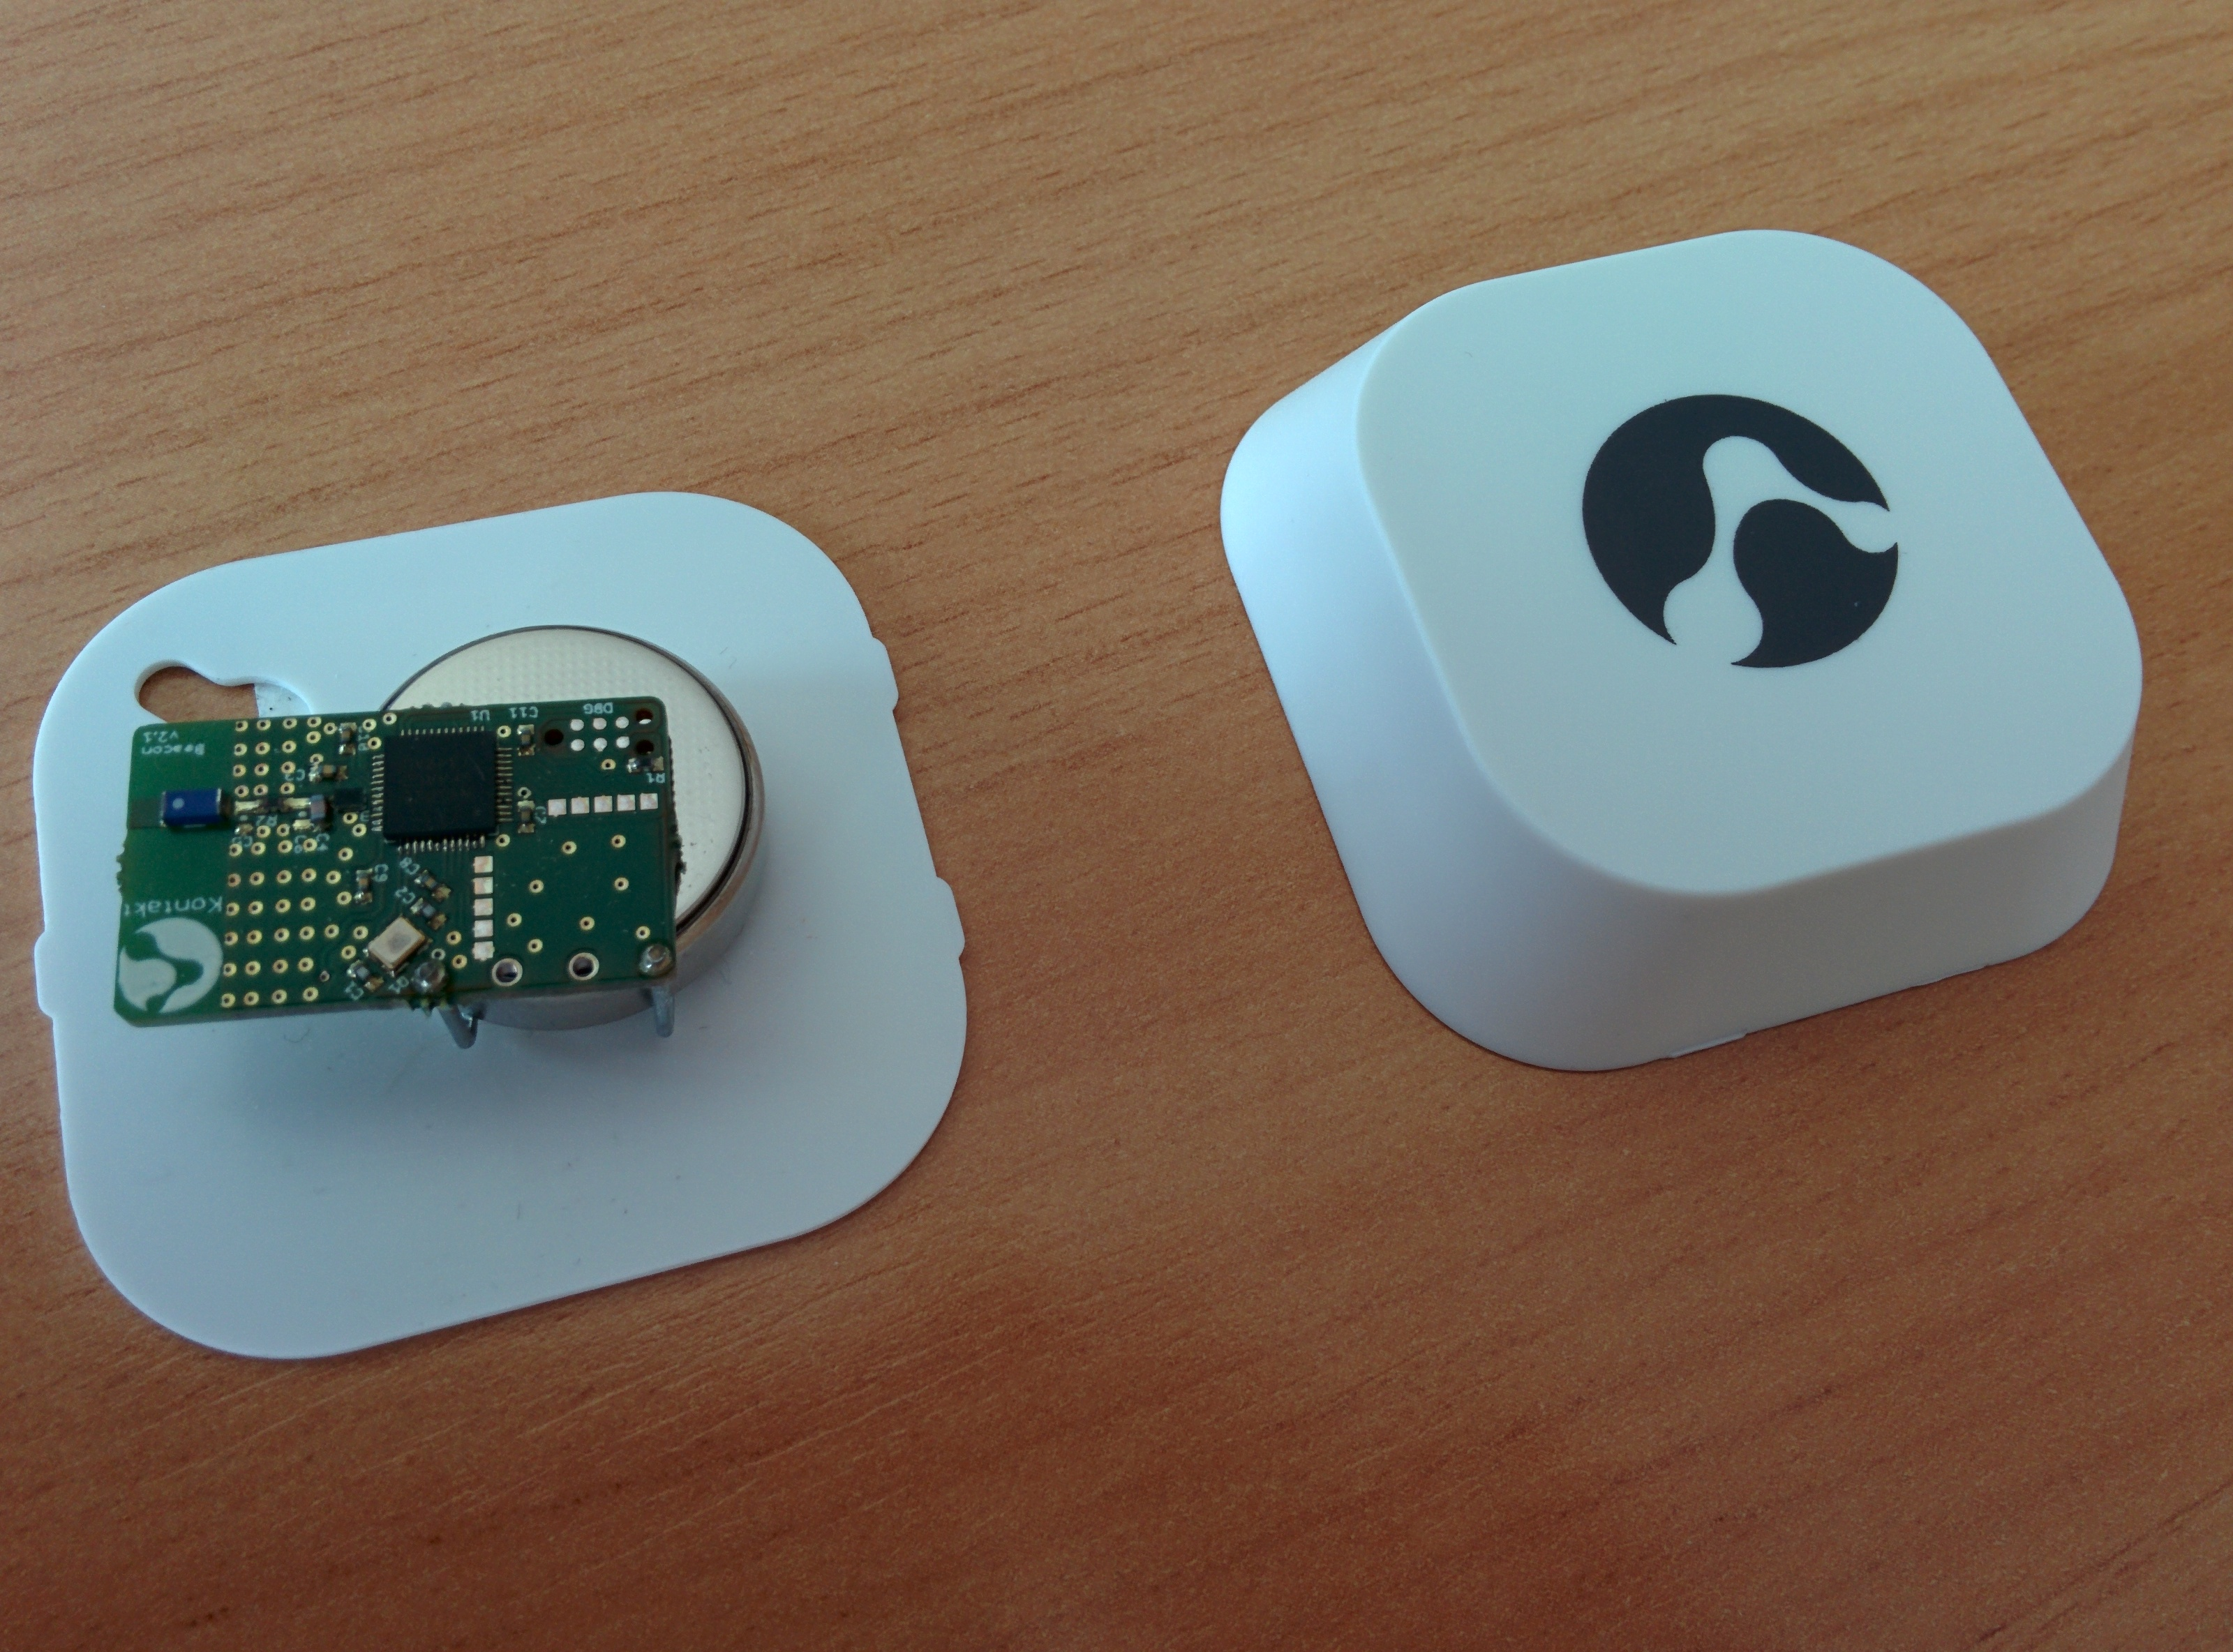
\includegraphics[scale=0.1]{pictures/IMG_20140505_095855}
    \caption{Kontakt.io iBeacon odašiljač}
\end{figure}

Dozvoljene vrijednosti jakosti odašiljanja su: $\SI{-30}{dBm}$, $\SI{-20}{dBm}$, $\SI{-16}{dBm}$, $\SI{-12}{dBm}$, $\SI{-8}{dBm}$, $\SI{-4}{dBm}$, $\SI{0}{dBm}$ i $\SI{4}{dBm}$.


\subsection*{Struktura paketa}
Uređaj odašilje dvije vrste paketa podataka: \textit{advertising} i \textit{scan response}.
\\
Tokom rada uređaj kontinuriano odašilje \textit{advertising} pakete i na taj obavještava okolne uređaje o svojoj prisutnosti. 
Drugi tip paketa, \textit{scan response} paket, šalje se odmah nakon \textit{advertising} paketa i sadrži dodatne informacije o odašiljaču, poput imena odašiljača, stanja baterije i slično.
\\

Struktura \textit{advertising} paketa odgovara strukturi iBeacon \textit{advertising} paketa navedenog u tablici \ref{tbl:iBeacon}, dok je struktura \textit{scan response} paketa navedena u tablici \ref{tbl:scanResponse}.
\\
%Prvih devet bajtova paketa su unaprijed poznate konstante (poput informacije o proizvođaču). Njih slijedi šesnaest bajtova koji čine proximity UUID, dva bajta za \textit{major} vrijednost, dva bajta za \textit{minor} vrijednost, a posljednji bajt predstavlja RSSI vrijednost (engl. \textit{Recived Signal Strength Indication}) izmjeren jedan metar od iBeacon uređaja.

\begin{table}[H]
    \centering
    \caption{Struktura \textit{scan response} paketa}
    \label{tbl:scanResponse}
    \begin{tabular}{ccc}
    \hline 
    Bajt & Vrijednost & Opis \\ 
    \hline 
    1. & 08* & Duljina podataka - 8 bajta \\ 
    2. & 09 & Tip podatka - Complete Local Name \\ 
    3. & 4B* & Lokalno ime uređaja \\ 
    4. & 6F* & Lokalno ime uređaja \\ 
    5. & 6E* & Lokalno ime uređaja \\ 
    6. & 74* & Lokalno ime uređaja \\ 
    7. & 61* & Lokalno ime uređaja \\ 
    8. & 6B* & Lokalno ime uređaja \\ 
    9. & 74* & Lokalno ime uređaja \\ 
    10. & 02 & Duljina podataka - 2 bajta \\ 
    11. & 0A & Tip podataka - Tx Power Value \\ 
    12. & F4 & Tx Power Value \\ 
    13. & 0A & Duljina podataka - 10 bajta \\ 
    14. & 16 & Tip podataka - service data \\ 
    15. & 0D & Service UUID 1. bajt \\ 
    16. & D0 & Service UUID 2. bajt \\ 
    17. & X & Identifikator odašiljača 1. bajt \\ 
    18. & X & Identifikator odašiljača 2. bajt \\ 
    19. & X & Identifikator odašiljača 3. bajt \\ 
    20. & X & Identifikator odašiljača 4. bajt \\ 
    21. & X & Firmware version 1. bajt \\ 
    22. & X & Firmware version 2. bajt \\ 
    23. & X & Razina baterije \\ 
    \hline
    %\multicolumn{3}{p{2pt}}X - vrijednosti ovise o postavkama konkretnog odašiljača \\
    %\multicolumn{3}{p{2pt}}* - varijabilne duljine, ovisi o duljini postavljenog imena odašiljača (max. 15 bajtova)
    \end{tabular}
    \caption*{
        X - vrijednosti ovise o postavkama konkretnog odašiljača \\
        * - varijabilne duljine, ovisi o duljini postavljenog imena odašiljača (max. 15 bajtova)
    } 
\end{table}

\chapter{Utvrđivanje relativne i apsolutne lokacije u zatvorenom prostoru}

Tehnologije navigacije i pozicioniranja koje se oslanjaju na udaljene satelite (poput GPS i GNSS tehnologija) nisu pogodne za korištenje u zatvorenim prostorima iz razloga što njihove signale apsorbiraju i reflektiraju krovovi, zidovi i ostali objekti u okolini. 
Iz istih razloga određivanje lokacije preko mobilnih signala, odnosno preko radio tornjeva nije moguće. 
\\
Stoga su za utvrđivanje lokacije u zatvorenom prostoru potrebni sasvim novi i drugačiji pristupi problemu te shodno tome, sasvim nove metode određivanja lokacije. 
Zbog ogromnog porasta pristupačnosti i popularnosti pametnih telefona, posljednjih nekoliko godina sve je veća potražnja za nekakvim pouzdanim rješenjem problema. 
Kako ne postoji nikakav \textit{de facto} standard, gotovo sva ponuđena rješenja su međusobno različita i koriste cijeli niz različitih tehnologija, od optičkih (npr. kamera uređaja) i radio (npr. signali obližnje bežične mreže) skroz do akustičnih tehnologija.
\\

Vjerojatno najznačajniji uspjeh je postignut sa praćenjem signala kojega odašilje obližnja bežična Wi-fi mreža. 
Velika prednost ove metode je značajan porast bežičnih pristupnih točaka na koje se mobilni i drugi uređaji mogu spojiti. 
Da bi se ovom metodom odredila lokacija uređaja potrebno je na neki način mapirati dotičnu pristupnu točku te zatim na temelju jakosti primljenog signala utvrditi poziciju mobilnog uređaja u odnosu na nju. 
Parametri mapiranja uključuju apsolutnu poziciju, SSID\footnote{\textit{service set identification}} i MAC\footnote{\textit{media access control address}} adresu pristupne točke (tj. WLAN uređaja). 
Neke od poznatijih web aplikacija poput WeFi\footnote{\url{http://www.wefi.com/maps/}} i WiGLE\footnote{\url{https://wigle.net}} sadrže više od sto milijuna mapiranih bežičnih pristupnih točaka. 
\\

\begin{figure}
    \centering
    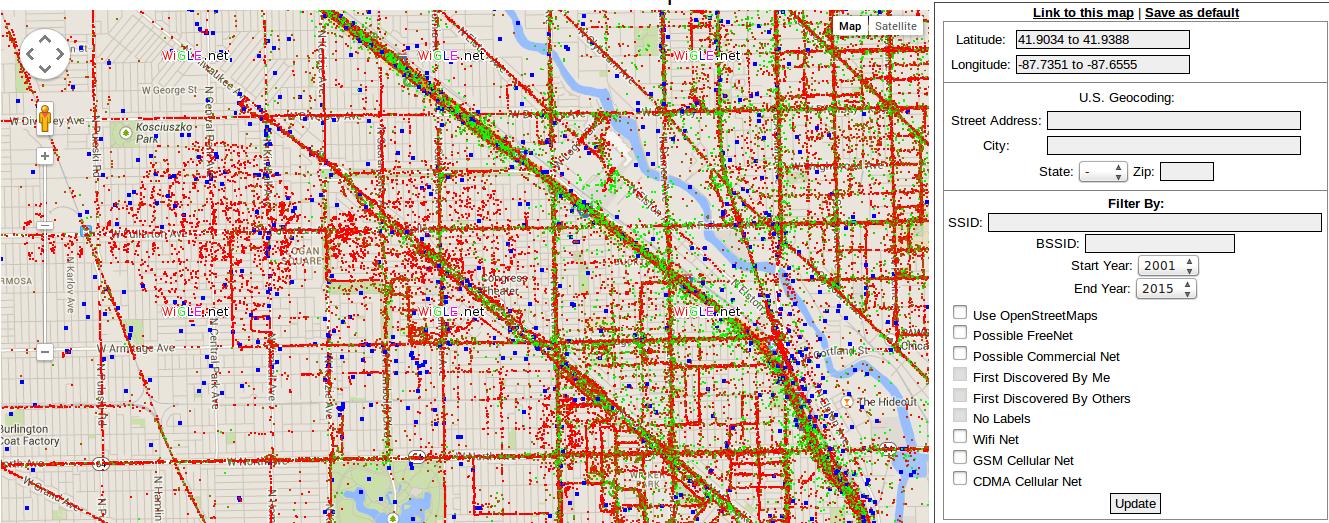
\includegraphics[scale=0.3]{pictures/WiGLE}
    \caption{WIGLE} % TODO caption
\end{figure}

Uz navigaciju i pozicioniranje pomoću Wi-fi mreža, dosta su popularne metode koje se služe tehnikama proširene i virtualne stvarnosti te tehnikama strojnog učenja, raspoznavanja uzoraka i računalnog vida. 
Jedna od popularnijih tehnika proširene i virtualne stvarnosti je korištenje posebnih oznaka (markera) kojega kamera mobilnog uređaja može prepoznati u prostoru. 
Vezano za metode strojnog učenja, raspoznavanja uzoraka i računalnog vida vjerojatno najistaknutiji i najambiciozniji projekt je projekt Tango\footnote{\url{https://www.google.com/atap/projecttango/}} kojega razvija tehnološki gigant Google. 
Cilj projekta je ponuditi rješenje koje će korištenjem kamere i ostalih senzora mobilnog uređaja nuditi pomoć pri navigaciji, pozicioniranju i prepoznavanju okoline, odnosno 3D mapiranje, u zatvorenom i otvorenom prostoru. 
Unatoč tome što je projekt još u ranoj fazi razvoja, razvojni tim je ostvario vidljiv napredak te su prvi prototipovi mobilnih uređaja već dostupni partnerima koji sudjeluju u razvoju.

\begin{figure}[H]
    \centering
    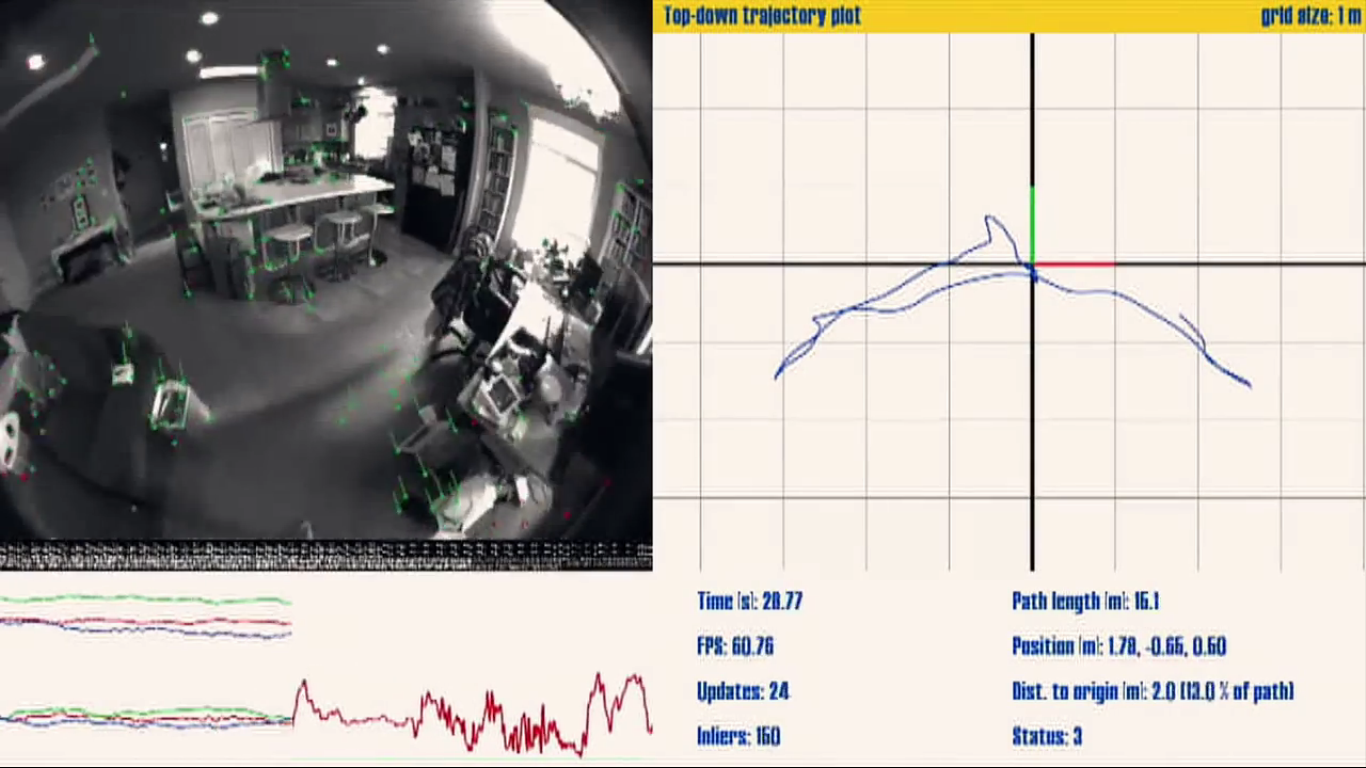
\includegraphics[scale=0.24]{pictures/tango1}
    \caption{Project Tango 1}
\end{figure}

\begin{figure}[H]
    \centering
    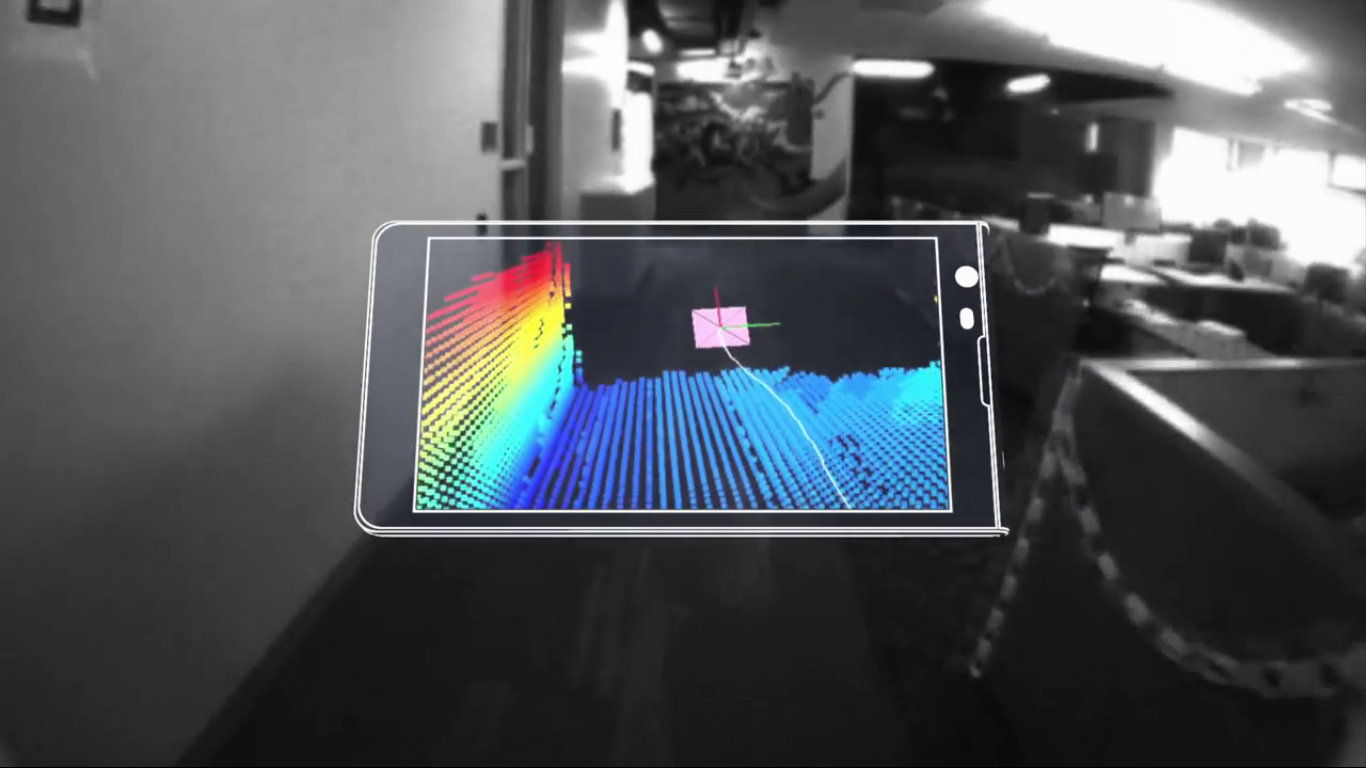
\includegraphics[scale=0.24]{pictures/tango2}
    \caption{Project Tango 2}
\end{figure}
%TODO referencirati youtube video u captionu

\section*{Utvrđivanje relativne udaljenosti od odašiljača}

blabla neki tekst.

%TODO postupak mjerenja, što sve treba, kako mjeriti, poteškoće
%TODO postupci: matematički, best fit curve, neuronska mreža i poteškoće, spomeniti genetsko programiranje
%TODO mjerenja udaljenosti
%TODO zaključak

\begin{table}[H]
    \centering
    \caption{Rezultat mjerenja signala u zatvorenom prostoru}
    \label{tbl:indoor}
	\begin{tabular}{|c|cccc||cccc|}%||cccc}
	\cline{2-9}
	\multicolumn{1}{!{\vrule width 0pt}c!{\vrule width 1pt}}{} & \multicolumn{4}{c||}{Beacon1} & \multicolumn{4}{c|}{Beacon2} \\ %& \multicolumn{4}{c}{Beacon3} \\ 
	\hline 
	Udaljenost & $\mu_{RSSI}$ & $\sigma_{RSSI}$ & $min_{RSSI}$ & $max_{RSSI}$ & $\mu_{RSSI}$ & $\sigma_{RSSI}$ & $min_{RSSI}$ & $max_{RSSI}$ \\ %& $\mu_{RSSI}$ & $\sigma_{RSSI}$ & $min_{RSSI}$ & $max_{RSSI}$ \\ 
	\hline 
	$0.5$ & $-81.075$ & $2.426$ & $-88$ & $-74$ & $-65.165$ & $2.546$ & $-76$ & $-56$ \\ %& -89.550 & 3.526 & -98 & -83 \\ 
	$1.0$ & $-80.320$ & $2.799$ & $-86$ & $-76$ & $-66.250$ & $2.316$ & $-73$ & $-59$ \\ %& -90.895 & 2.101 & -96 & -86 \\ 
	$1.5$ & $-75.575$ & $3.298$ & $-80$ & $-70$ & $-62.695$ & $4.324$ & $-69$ & $-57$ \\ %& -91.350 & 3.162 & -101 & -86 \\ 
	$2.0$ & $-73.990$ & $2.558$ & $-79$ & $-68$ & $-58.750$ & $1.982$ & $-62$ & $-53$ \\ %& -91.695 & 2.134 & -99 & -86 \\ 
	$2.5$ & $-78.725$ & $0.907$ & $-81$ & $-74$ & $-63.595$ & $0.875$ & $-66$ & $-59$ \\ %& -89.630 & 1.583 & -99 & -86 \\ 
	$3.0$ & $-82.470$ & $4.053$ & $-91$ & $-74$ & $-67.810$ & $2.619$ & $-73$ & $-62$ \\ %& -93.385 & 2.156 & -100 & -88 \\ 
	$3.5$ & $-81.685$ & $2.892$ & $-87$ & $-77$ & $-71.620$ & $3.537$ & $-80$ & $-65$ \\ %& - & - & - & - \\ 
	$4.0$ & $-83.115$ & $1.903$ & $-88$ & $-77$ & $-68.720$ & $2.000$ & $-73$ & $-65$ \\ %& - & - & - & - \\ 
	$4.5$ & $-91.125$ & $3.057$ & $-98$ & $-85$ & $-74.975$ & $3.065$ & $-81$ & $-68$ \\ %& - & - & - & - \\ 
	$5.0$ & $-88.705$ & $2.198$ & $-93$ & $-83$ & $-72.445$ & $3.485$ & $-78$ & $-65$ \\ %& - & - & - & - \\ 
	$5.5$ & $-88.935$ & $3.487$ & $-97$ & $-83$ & $-79.920$ & $6.883$ & $-93$ & $-68$ \\ %& - & - & - & - \\ 
	$6.0$ & $-92.450$ & $2.399$ & $-99$ & $-87$ & $-82.175$ & $5.896$ & $-98$ & $-71$ \\ %& - & - & - & - \\ 
	$6.5$ & $-93.610$ & $1.691$ & $-99$ & $-90$ & $-74.085$ & $2.977$ & $-80$ & $-68$ \\ %& - & - & - & - \\ 
	$7.0$ & - & - & - & - & $-71.700$ & $2.858$ & $-77$ & $-65$ \\ %& - & - & - & - \\ 
	$7.5$ & - & - & - & - & $-76.065$ & $2.241$ & $-80$ & $-71$ \\ %& - & - & - & - \\ 
	$8.0$ & - & - & - & - & $-78.295$ & $4.926$ & $-91$ & $-71$ \\ %& - & - & - & - \\ 
	\hline 
	\end{tabular}
\end{table}


\section*{Utvrđivanje apsolutne lokacije}
%TODO općenito o utvrđivanju apsolutne lokacije

\subsection*{Triangulacija}

Postupak triangulacije
%TODO objasniti postupak triangulacije
%TODO matematički postupak kod triangulacije
%TODO iBeacon i triangulacija

\subsection*{Trilateracija}
%TODO objasniti postupak trilateracije
%TODO matematički postupak trilateracije
%TODO iBeacon i trilateracija

\chapter{Radno okruženje Apache Cordova}

Radno okruženje Apache Cordova je skup aplikacijsko programskih sučelja \engl{application programming interface, API} koji omogućavaju da razvijatelj mobilnih aplikacija pristupa osnovnim funkcijama mobilnoga uređaja, poput kamere, sustava za pohranu podataka i telefonskog imenika preko JavaScript jezika. 
U kombinaciji sa radnim okruženjima poput Sencha Touch, Dojo Mobile i Ionic aplikacije za pametne telefone mogu se razvijati korištenjem samo HTML, CSS i JavaScript programskog jezika.
\\

Korištenjem Apache Cordove programer je oslobođen pisanja aplikacija u nativnim jezicima uređaja (npr. Java za Android, Objective-C za iOS), već se koriste isključivo prethodno spomenute web tehnologije. 
Bez obzira na to što aplikacije nisu napisane u nativnim jezicima, Apache Cordova aplikacije se prevode i pakiraju pomoću SDK \engl{software development kit, SDK} željene platforme stoga se aplikacije mogu i postaviti na trgovine aplikacija \engl{app store} dotične platforme. 
\\

Cordova nudi skup uniformnih JavaScript biblioteka čije funkcije programer može pozivati. 
One imaju podršku za povezivanje sa specifičnim platformama. Cordova je trenutno dostupna za sljedeće platforme: Android, iOS, Blackberry,Windows Phone, Palm WebOS, Bada i Symbian.
\\
Službene Cordova JavaScript biblioteke navedene su u \ref{cordovaLib}, dok je oko dvije stotine dodatnih biblioteka dostupno na službenom repozitoriju\footnote{\url{http://plugins.cordova.io}}. %TODO srediti \ref{cordovaLib} 
\\
Za pristup \textit{Bluetooth Low Energy} funkcijama mobilnog uređaja korištena je \textbf{Cordova BLE} biblioteka\footnote{\url{https://github.com/evothings/cordova-ble}}.
\\

\fbox{
\begin{minipage}{0.9\textwidth}
\begin{description}[style=nextline]
        \label{cordovaLib}
        \captionof{figure}{Službene Cordova biblioteke}
	    \item[Battery Status]
	        Omogućava nadgledanje stanja baterije uređaja.
	    \item[Camera]
	        Omogućava pristup kameri uređaja.
	    \item[Contacts]
	        Omogućava pristup telefonskom imeniku uređaja.
	    \item[Device]
	        Omogućava pristup specifičnim informacijama uređaja (npr. ime uređaja, operacijski sustav).
	    \item[Device Motion (Accelerometer)]
	        Omogućava pristup senzoru ubrzanja (akcelerometar).
	    \item[Device Orientation (Compass)]
	        Omogućava pristup kompasu uređaja.
	    \item[Dialogs]
	        Omogućava korištenje sustava obavijesti uređaja.
	    \item[FileSystem]
	        Omogućava korištenje datotečnog sustava uređaja.
	    \item[FileTransfer]
	        Omogućava pristup sustavu za prijenos datoteka.
	    \item[Geolocation]
	        Omogućava pristup prema geolokacijskom sustavu. 
	    \item[Globalizationg]
	        Omogućava različite reprezentacije objekata ovisno o postavkama lokacije uređaja.
	    \item[InAppBrowser]
	        Omogućava otvaranje URL-ova u novoj instanci web-preglednika uređaja.
	    \item[Media]
	        Omogućava snimanje i reprodukciju audio datoteka.
	    \item[Media Capture]
	        Omogućava snimanje audio i video datoteka.
	    \item[Network Information (Connection)]
	        Omogućava pristup informacijama o stanju mreže uređaja.
	    \item[Splashscreen]
	        Omogućava manipuliranje početnog zaslona aplikacije.
	    \item[Vibration]
	        Omogućava korištenje mehanizma za vibriranje uređaja.
    \end{description}
\end{minipage}
}    

\section*{Radno okruženje Ionic}

Ionic je radno okruženje napisano sa HTML, CSS i JavaScript programskim jezikom čiji je cilj olakšati razvoj hibridnih mobilnih aplikacija\footnote{Aplikacije napravljene korištenjem web tehnologija. 
Pokreću se unutar posebnog spremnika uređaja te koriste funkcije web preglednika za prikaz HTML sadržaja i izvođenje JavaScript k\^oda} stoga je ono jako dobar izbor prilikom izrade Cordova aplikacija. 
Ionic je primarno okrenut prema olakšanju izrade korisničkog sučelja, odnosno nudi cijeli niz funkcija koje razvijatelju olakšavaju izradu velikih i složenih mobilnih aplikacija. 
U pozadini, Ionic koristi danas sve popularnije JavaScript \textit{frontend} radno okruženje AngularJS koje je namjenjeno izradi \textit{single-page} web aplikacija. 
Korištenjem AngularJSa u Ionic je dodan cijeli niz direktiva\footnote{Posebne oznake DOM elemenata koje obavještavaju AngularJS HTML prevoditelja da transformira elemente ili im doda novo ponašanje.}, filtera\footnote{Funkcije za obradu ili transformaciju podataka koji se prikazuju korisniku. 
Npr. mogu se koristiti za abecedni prikaz elemenata liste, prikaz teksta isključivo velikim slovom itd.}, servisa\footnote{Jedinstveni objekti \engl{singleton} koji se koriste za dijeljenje funkcija i resursa unutar aplikacije.} i drugih funkcija koje programeru rješavaju cijeli niz problema poput osjetljivog dizajna \engl{responsive design}, hvatanja raznih korisnikovih interakcija (dodiri s jedim ili više prstiju, povlačenje \engl{swipe} stavki, stezanju i širenju stavki \engl{pinch} i cijeli niz drugih). 
\\

Ionic se sastoji od dva temeljna dijela. 
Prvi dio čine CSS i Sass datoteke čija je svrha da razvijateljima olakšaju izradu vizualnoga dizajna aplikacije. 
Drugi dio čine JavaScript datoteke i HTML predlošci koji pojednostavljuju izradu aplikacija složene arhitekture te programerima nude cijeli niz pomoćnih funkcija.
\\

Ionic je relativno novo radno okruženje i u vrijeme pisanja ovog rada je u beta verziji. 
Unatoč tome, veliki broj funkcija već je implementiran i samo njihovim korištenjem mogu se napraviti velike, složene i vizualno privlačne mobilne aplikacije. 
Uz to, Ionic je izdan pod MIT licencom i njegov izvorni kod je javno dostupan na službenom Github repozitoriju\footnote{\url{https://github.com/driftyco/ionic}}.

\chapter{Praktični rad}

U iBeacon poglavlju spomenuto je kako se tehnologija iBeacon može iskoristiti u gotovo svim situacijama gdje se sadržaj mijenja ovisno o kontekstu prostora, npr. trgovinama, muzejima, bolnicama i sličnim objektima. 
\\
U nastavku poglavlja opisano je kako se tehnologija iBeacon može integrirati u trgovine. 
\\

Za integraciju je potrebno imati postavljene iBeacon uređaje u prostoru, klijentsku mobilnu aplikaciju koja može prepoznati BLE, odnosno iBeacon, odašiljače te poslužiteljsku aplikaciju s koje će mobilni uređaj dohvaćati relevantne podatke.  

\section*{Poslužiteljska aplikacija}

Spree Commerce (u daljnjem tekstu Spree) je elektronička trgovina \engl{e-commerce} otvorenog koda napisana u Ruby on Rails radnom okruženju. 
Rad na Spreeu je počeo 2007. godine, a danas je jedna od najpopularnijih platformi za elektroničku trgovinu. 
Trenutno više od 45 tisuća trgovina koristi Spree. %TODO reff http://spreecommerce.com/storefront 
\\
Odlike Spree rješenja su ogroman broj već implementiranih funkcija koje imaju sve moderne elektroničke trgovine, modularan programski kôd, lakoća dodavanja novih funkcionalnosti te izmjena i konfiguracija postojećih te brojne druge. 
Uz to, za gotovo svaki aspekt sustava dostupan je skup aplikacijsko programskih sučelja što pojednostavljuje integraciju sustava sa drugim tehnologijama (poput integracije sa mobilnim platformama).
\\

\begin{figure}[H]
    \centering
    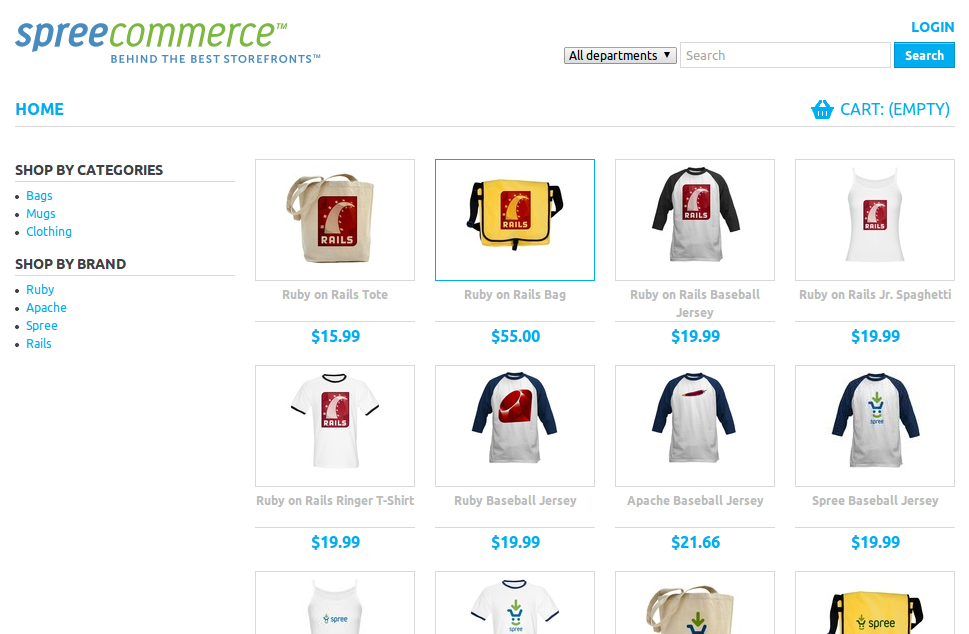
\includegraphics[scale=0.40]{pictures/spree}
    \caption{Početni ekran Spree korisničkog sučelja}
    \label{pic:spree}
\end{figure}

\begin{figure}[H]
    \centering
    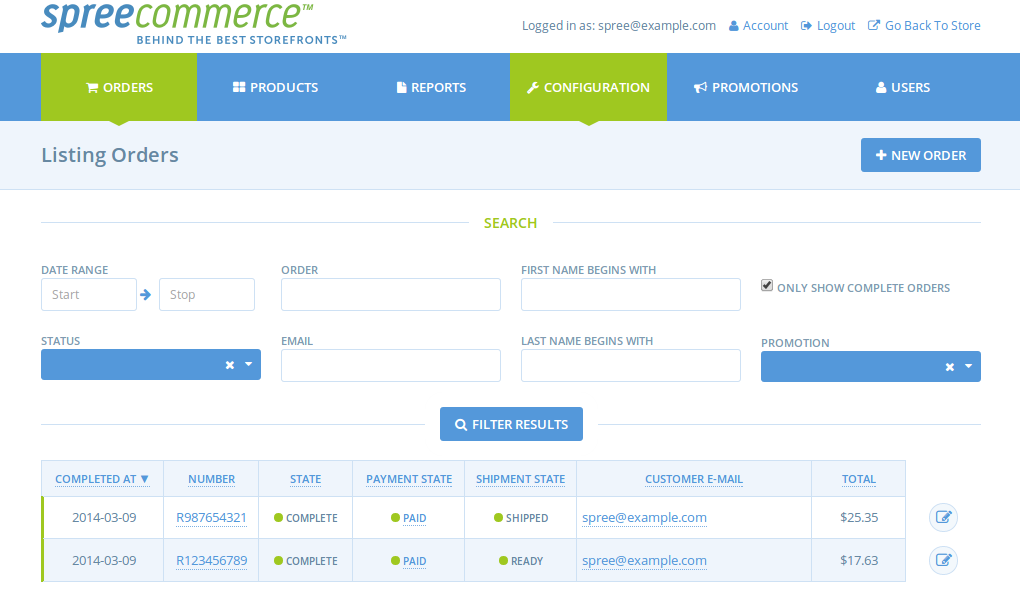
\includegraphics[scale=0.40]{pictures/spree_admin}
    \caption{Početni ekran Spree administratorskog sučelja}
    \label{pic:spree}
\end{figure}

\begin{figure}[H]
    \centering
    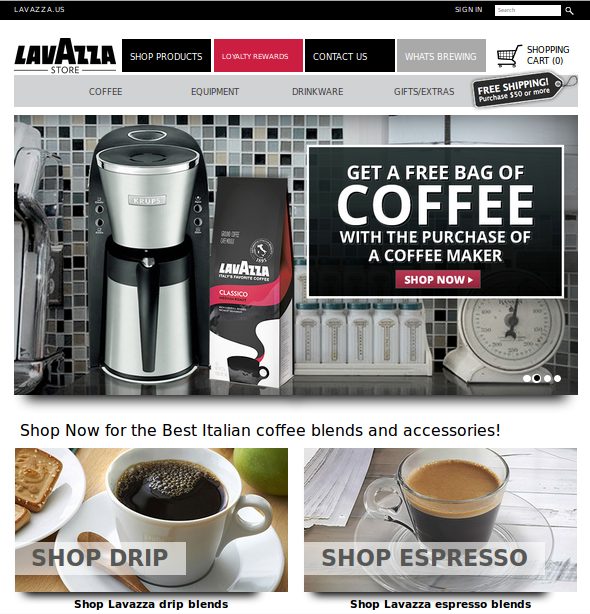
\includegraphics[scale=0.65]{pictures/spree_lavazza}
    \caption{Lavazza Store - jedna od mnogobrojnih elektroničkih trgovina koje koriste Spree}
    \label{pic:spreeLavazza}
\end{figure}

Spree je podijeljen na nekoliko ključnih komponenti (tj. Ruby Gemova):
\begin{description}[style=nextline]
    \item[spree\_api] Skup aplikacijsko programskih sučelja koji zadovoljavaju REST\footnote{\textit{Representational State Transfer}, \url{http://en.wikipedia.org/wiki/Representational_state_transfer}} principe.
    \item[spree\_frontend] Komponente korisničkog sučelja.
    \item[spree\_backend] Komponente korisničkog sučelja administratora aplikacije.
    \item[spree\_cmd] Komponente sučelja naredbenog retka \engl{command-line interface, CLI}.
    \item[spree\_core] Ključne komponente, sadrži veliku većinu poslovne logike.
    \item[spree\_sample] Primjeri podataka.
\end{description}

Ako programer želi dodati neku od Spree komponenti u svoju postojeću aplikaciju, sve što treba napraviti je dodati željene komponente u Gemfile\footnote{datoteka koja sadrži popis svih Ruby Gemova koji se koriste u projektu} te pokrenuti instalaciju.

%TODO instalacija railsa i spreea 


%TODO dijelovi spreea
%TODO spree_taxon_web_services
%TODO instalacija aplikacije
%TODO pokretanje aplikacije

\section*{Klijentska aplikacija}

%TODO uvod
%TODO integriranje aplikacije sa ibeaconima, use caseovi
%TODO spajanje aplikacije sa serverom
%TODO instalacija i pokretanje aplikacije
%TODO eksperimentalna aplikacija

\chapter{Zaključak}
Zaključak.

\nocite{*}
\bibliography{literatura}
\bibliographystyle{fer}

\begin{sazetak}

Tehnologije navigacije i pozicioniranja koje se oslanjaju na udaljene satelite (npr. GPS tehnologija) nisu pogodne za korištenje u zatvorenim prostorima. 
Stoga su za utvrđivanje lokacije u zatvorenom prostoru potrebne nove i drugačije metode. 
Kako ne postoji nikakav \textit{de facto} standard, danas postoji niz različitih rješenja. 
Uvođenjem Bluetooth 4.0 specifikacije i tehnologije Bluetooth Low Energy dolazi do razvoja niza jeftinih uređaja koji se mogu iskoristiti za rješavanje problema određivanja lokacije. 
Kako na signal u zatvorenom prostoru djeluje veliki broj smetnji određivanje lokacije pomoću BLE tehnologije nije precizno i preporuča se korištenje samo za određivanje okvirne lokacije. 
Unatoč tome, ono se može primijeniti u gotovo svim situacijama gdje se sadržaj mijenja ovisno o kontekstu prostora stoga se ono danas sve više integrira u mobilne aplikacije. 
%Razvojem radnih okruženja za izradu hibridnih mobilnih aplikacija, izrada mobilnih aplikacija za više platformi postaje jednostavnija, a

\kljucnerijeci{Bluetooth, BLE, mikrolokacija, iBeacon, Android, iOS, Apache Cordova, Ruby on Rails, Ruby, JavaScript, razvoj mobilnih aplikacija}
\end{sazetak}

\engtitle{Determining a micro-location of a mobile device}
\begin{abstract}
%Positioning technologies that receive signals from distant satellites (such as GPS) are unusable indoors. 

\keywords{Bluetooth, BLE, mikrolokacija, iBeacon, Android, iOS, Apache Cordova, Ruby on Rails, Ruby, JavaScript, mobile development}
\end{abstract}

\end{document}